\documentclass[a4paper,11pt]{article}
\usepackage[utf8]{inputenc}
\usepackage[normalem]{ulem}
\usepackage{graphicx, hyperref, caption, amsmath, amssymb, amsthm, subcaption, tabularx, float, fullpage, url,dsfont, tipa, textcomp, braket, physics, grffile, color,  multicol,wasysym,slantsc, url, color}
\usepackage[dutch]{babel}
\usepackage{graphicx}
\usepackage{listings,caption,subcaption}
\usepackage[margin=2cm]{geometry}
\usepackage[dvipsnames]{xcolor}
%\usepackage{preamble}
\usepackage{enumitem}
\usepackage{gensymb}
\usepackage{circuitikz}
\usetikzlibrary{patterns}
\usetikzlibrary{decorations.pathmorphing,patterns}

\newcommand{\stkout}[1]{\ifmmode\text{\sout{\ensuremath{#1}}}\else\sout{#1}\fi}

%\usepackage{subcaption}
%%%%%%%%%%%%%%%%%%%%%%%%%%%%%%%%%%%%%%%%
\title{Examen AN1}


\begin{document}

\section*{Optie 1: Staafje \& schijf}
\subsection*{Opgave}
Een schijfje met puntmassa $m_1$ en een massieve staaf met lengte $\ell=4d$ en massa $m_2$ liggen op een wrijvingsloze tafel. Het schijfje vliegt met een snelheid $v_0 \hat{j}$ in de $y$-richting tegen de staaf, die in de richting van de $x$-as gepositioneerd is (zie figuur \ref{fig:VoorBotsing}). Als het schijfje de staaf raakt op een afstand $d$ van de midden, dan zal het schijfje verder bewegen met snelheid $\vec{v}_1$ en de staaf met een lineaire snelheid $\vec{v}_2$. Verder zal de staaf ook beginnen roteren (zie figuur \ref{fig:NaBotsing}). De richtingen van $\vec v_1$ en $\vec v_2$ op deze tekeningen zijn willekeurig gekozen. Als je aanneemt dat er behoud van energie is tijdens de botsing toon dan aan dat:
\begin{enumerate}[label=(\alph*)]
	\item $\vec{v}_1$ voldoet aan
	\begin{equation}
		v_0^2=v_{1,x}^2+v_{1,y}^2+\alpha v_{1,x}^2+\alpha(v_0-v_{1,y})^2+3\alpha(v_0-v_{1,y})^2
	\end{equation}
	waar $\alpha=m_1/m_2$.
	\item Toon aan dat gegeven een $v_{1,x}$, er precies twee oplossingen zijn voor $v_{1,y}$ als en slechts als
	\begin{equation}
		v_0^2>(1+4\alpha)(1+\alpha)v_{1,x}^2.
	\end{equation}
	\item Nu gaan we voor de gemakkelijkheid aannemen dat $v_{1,x}=0$. Er zijn nu twee mogelijke oplossingen voor $v_{1,y}$. De eerste is wanneer het schijfje dwars door de staaf gaat en ze elkaar dus niet zouden raken. Wat is de andere oplossing?
\end{enumerate}
\begin{figure}[H]
	\centering
	\begin{subfigure}[b]{0.45\textwidth}
		\centering
		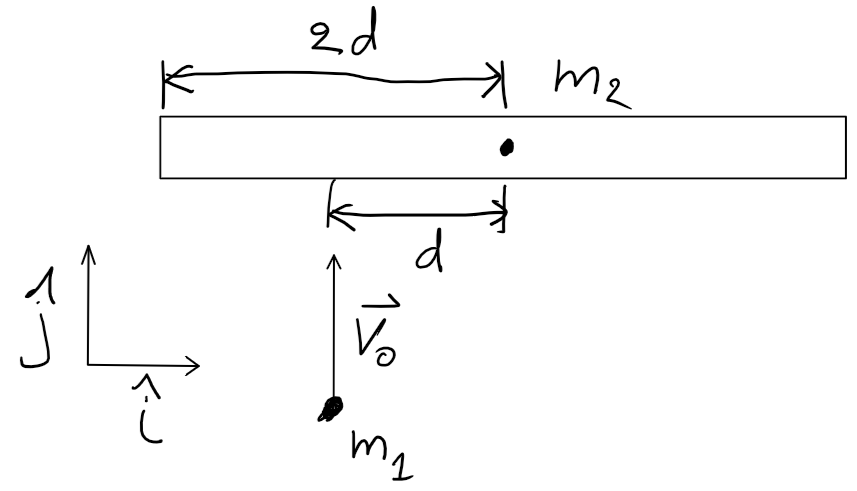
\includegraphics[width=\textwidth]{VoorBotsing}
		\caption{}
		\label{fig:VoorBotsing}
	\end{subfigure}
	\hfill
	\begin{subfigure}[b]{0.45\textwidth}
		\centering
		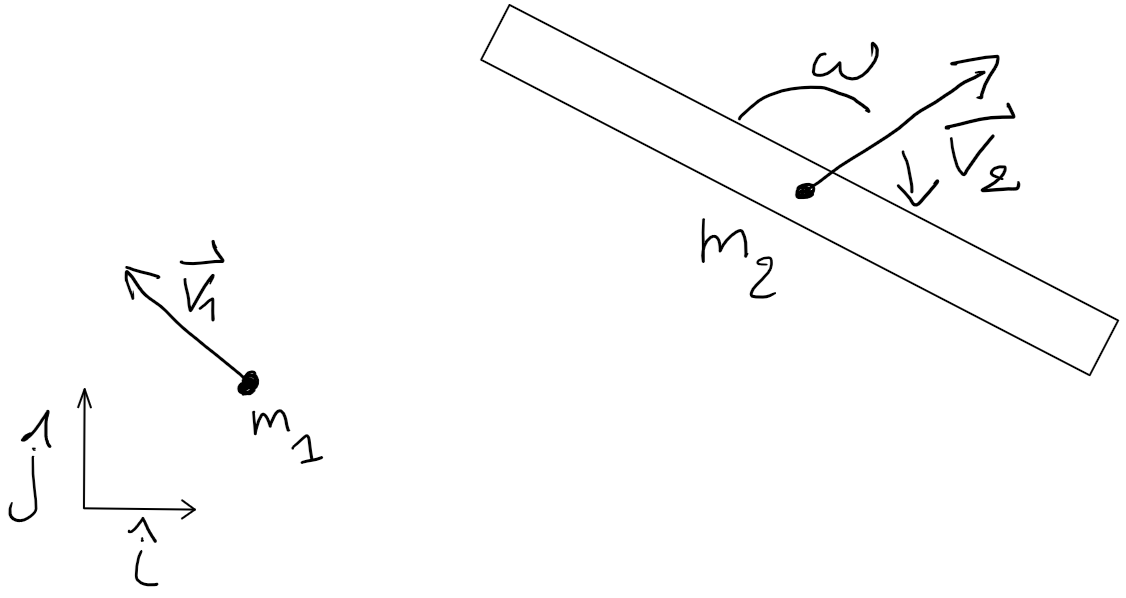
\includegraphics[width=\textwidth]{NaBotsing}
		\caption{}
		\label{fig:NaBotsing}
	\end{subfigure}
	\caption{Figuur \ref{fig:VoorBotsing} geeft de situatie voor de botsing weer en figuur \ref{fig:NaBotsing} die na de botsing.}
	\label{fig:Botsing}
\end{figure}

\subsection*{Oplossing}
Behoud van energie, momentum in de $x$-richting, momentum in de $y$-richting en angular momentum zijn gegeven door
\begin{align}
	\frac{m_1 v_0^2}{2}&=\frac{m_1v_{1,x}^2}{2}+\frac{m_1v_{1,y}^2}{2}+\frac{m_2v_{2,x}^2}{2}+\frac{m_2v_{2,y}^2}{2}+\frac{I\omega^2}{2}\\
	m_1v_0&=m_1v_{1,y}+m_2v_{2,y}\\
	0&=m_1v_{1,x}+m_2v_{2,x}\\
	m_1dv_0&=I\omega+m_1dv_{1,y}
\end{align}
respectievelijk. Gebruikmaken van het feit dat $I=\frac{1}{3}d^2m_2$ en invullen dat $\alpha=\frac{m_1}{m_2}$ geeft
\begin{align}
	\alpha v_0^2&=\alpha v_{1,x}^2+\alpha v_{1,y}^2+v_{2,x}^2+v_{2,y}^2+\frac{1}{3}d^2\omega^2\\
	\alpha v_0&=\alpha v_{1,y}+v_{2,y}\\
	0&=\alpha v_{1,x}+v_{2,x}\\
	3\alpha v_0&=d\omega+\alpha v_{1,y}.
\end{align}
Als je nu de laatste drie vergelijkingen gebruikt en invult in de eerste (en dus alles schrijft in functie van $\vec{v}_1$) krijg je
\begin{align}
	\alpha v_0^2&=\alpha v_{1,x}^2+\alpha v_{1,y}^2+\alpha^2 v_{1,x}^2+\alpha^2(v_0-v_{1,y})^2+3\alpha^2(v_0-v_{1,y})^2\\
	v_0^2&=v_{1,x}^2+v_{1,y}^2+\alpha v_{1,x}^2+\alpha(v_0-v_{1,y})^2+3\alpha(v_0-v_{1,y})^2\\
	v_0^2&=v_{1,x}^2+v_{1,y}^2+\alpha v_{1,x}^2+\alpha(v_0^2-2v_0v_{1,y}+v_{1,y}^2)+3\alpha(v_0^2-2v_0v_{1,y}+v_{1,y}^2).
\end{align}
Hieruit lezen we af
\begin{align}
	a&=1+4\alpha \\ b&=-8\alpha v_0 \\ c&=(1+\alpha)v_{1,x}^2+(4\alpha-1)v_0^2.
\end{align}
Dit geeft:
\begin{align}
	D&=64\alpha^2v_0^2-4(1+4\alpha)((1+\alpha)v_{1,x}^2+(4\alpha-1)v_0^2)\\
	&=64\alpha^2v_0^2-4((1+4\alpha)(1+\alpha)v_{1,x}^2+(1+4\alpha)(4\alpha-1)v_0^2)\\
	&=\stkout{64\alpha^2v_0^2}-4((1+4\alpha)(1+\alpha)v_{1,x}^2+(1-\stkout{16\alpha^2})v_0^2)\\
	&=4v_0^2-4(1+4\alpha)(1+\alpha)v_{1,x}^2.
\end{align}
Dus we krijgen dat er twee mogelijke oplossingen zijn voor $v_{1,y}$ als en slechts als
\begin{equation}
	v_0^2>(1+4\alpha)(1+\alpha)v_{1,x}^2.
\end{equation}
Dit vind ik een kei logische uitkomst omdat je inderdaad verwacht dat er alleen oplossingen zijn als $v_0$ groot is ten opzichte van $v_{1,x}$. Ook, als $v_{1,x}=0$ genomen wordt zijn er oplossingen voor elke $\alpha$ wat je inderdaad zou verwachten. Nu zullen we in de volgende deelvraag aannemen dat $v_{1,x}=0$. Dan verwachten we dat er twee oplossingen zijn, namelijk
\begin{align}
	v_{1,y}&=\frac{8\alpha v_0-2v_0}{2+8\alpha}=\frac{1-4\alpha}{1+4\alpha}v_0&v_{1,y}&=\frac{8\alpha v_0+2v_0}{2+8\alpha}=v_0.
\end{align}
De tweede oplossing komt voor wanneer het bolletje dwars door de staaf vliegt (dat hebben we nog niet uitgesloten) de eerste oplossing is de niet triviale oplossing wanneer er een raking is.
\newpage 
\section*{Optie 2: Veren en evenwicht}
\subsection*{Opgave}
Een dunne staaf van lengte $L$ en massa $M$ is aan de rechterkant verbonden met het plafond via aan een lineaire veer (veerconstane $k$). Aan de linkerkant is de staaf verbonden met een muur, waarbij een torsieveer (angulaire veerconstante $\kappa$) dienst doet als scharnier. Dit systeem is in evenwicht wanneer de staaf horizontaal is, zoals getekend in figuur \ref{fig:veren}. In dit geval heeft de lineare veer een uitrekking $y_0$ t.o.v. zijn rustlengte, en de torsieveer een uitwijkingshoek $\theta_0$. 
\\ \\
Wanneer de staaf onder een kleine hoek $\theta$ uit de evenwichtspositie gehaald wordt, vindt er een oscillatie plaats bij het loslaten. Leid de frequentie $f$ af van deze oscillatiebeweging als een functie van $M$, $L$, $k$ en $\kappa$.

\subsection*{Extra uitleg}
\begin{itemize}
    \item Het traagheidsmoment van een dunne staaf rond zijn massamiddelpunt is:
\begin{equation}
    I=\frac{1}{12}ML^2.
\end{equation}
    \item  Een torsieveer (figuur \ref{fig:torsieveer}) is het angulair equivalent van de gekende, lineaire veer. Dit type veer veroorzaakt een krachtmoment $\tau$ volgens de angulaire wet van Hooke:
    \begin{equation}
       \tau = -\kappa \theta,
    \end{equation}
    waarbij $\kappa$ de angulaire veerconstante is met eenheden ${\rm N\, m/rad }$ en $\theta$ de openingshoek t.o.v. de rusthoek.
    \end{itemize}

\begin{figure}[H]
    \centering
    \begin{subfigure}{0.45\textwidth}
        \begin{circuitikz}
        
        % Vertical wall
        \fill[pattern=north east lines] (0,3) rectangle (0.25,5);
        \draw (0.25,3) -- (0.25,5);
        
         % Horizontal wall
        \fill[pattern=north east lines] (3.5,7.75) rectangle (4.5,8);
        \draw (3.5,7.75) -- (4.5,7.75);
        
        % Torsion spring & rod
        \node[circle,draw] (c) at (0.425,3.965){};
        \node at (0.55,3.65){$\kappa$};
        \draw[fill=gray!35] (0.6,4.02) rectangle (4,3.92) node[midway,above]{$M$} ;
        
        % Regular spring
        \draw[decoration={aspect=0.7, segment length=3mm, amplitude=1.2mm,pre length = 1mm, post length =0.3mm,coil},decorate](4,7.75) -- (4,4) node[midway, right]{$k$};
        
        % Connection points
        \filldraw (4,3.98) circle (1pt);
        \filldraw (4,7.75) circle (1pt);
        
        % Measurements
        \draw[<->] (0.6,3.3) -- (4,3.3) node[midway, below] {$L$};
        \draw[|->] (4.75,5) -- (4.75,4) node[midway,right] {$y_0$};
        
        \draw (0.55,4.15) -- (1.1,4.7);
        \draw[<-] (1.1,4.1) arc [start angle=0, end angle=45, x radius=0.5, y radius=0.5] node[midway,right] {$\theta_0$};
        
        \end{circuitikz}
    \caption{Opstelling}
    \label{fig:veren}
    \end{subfigure}
    \begin{subfigure}{0.45\textwidth}
        \centering
        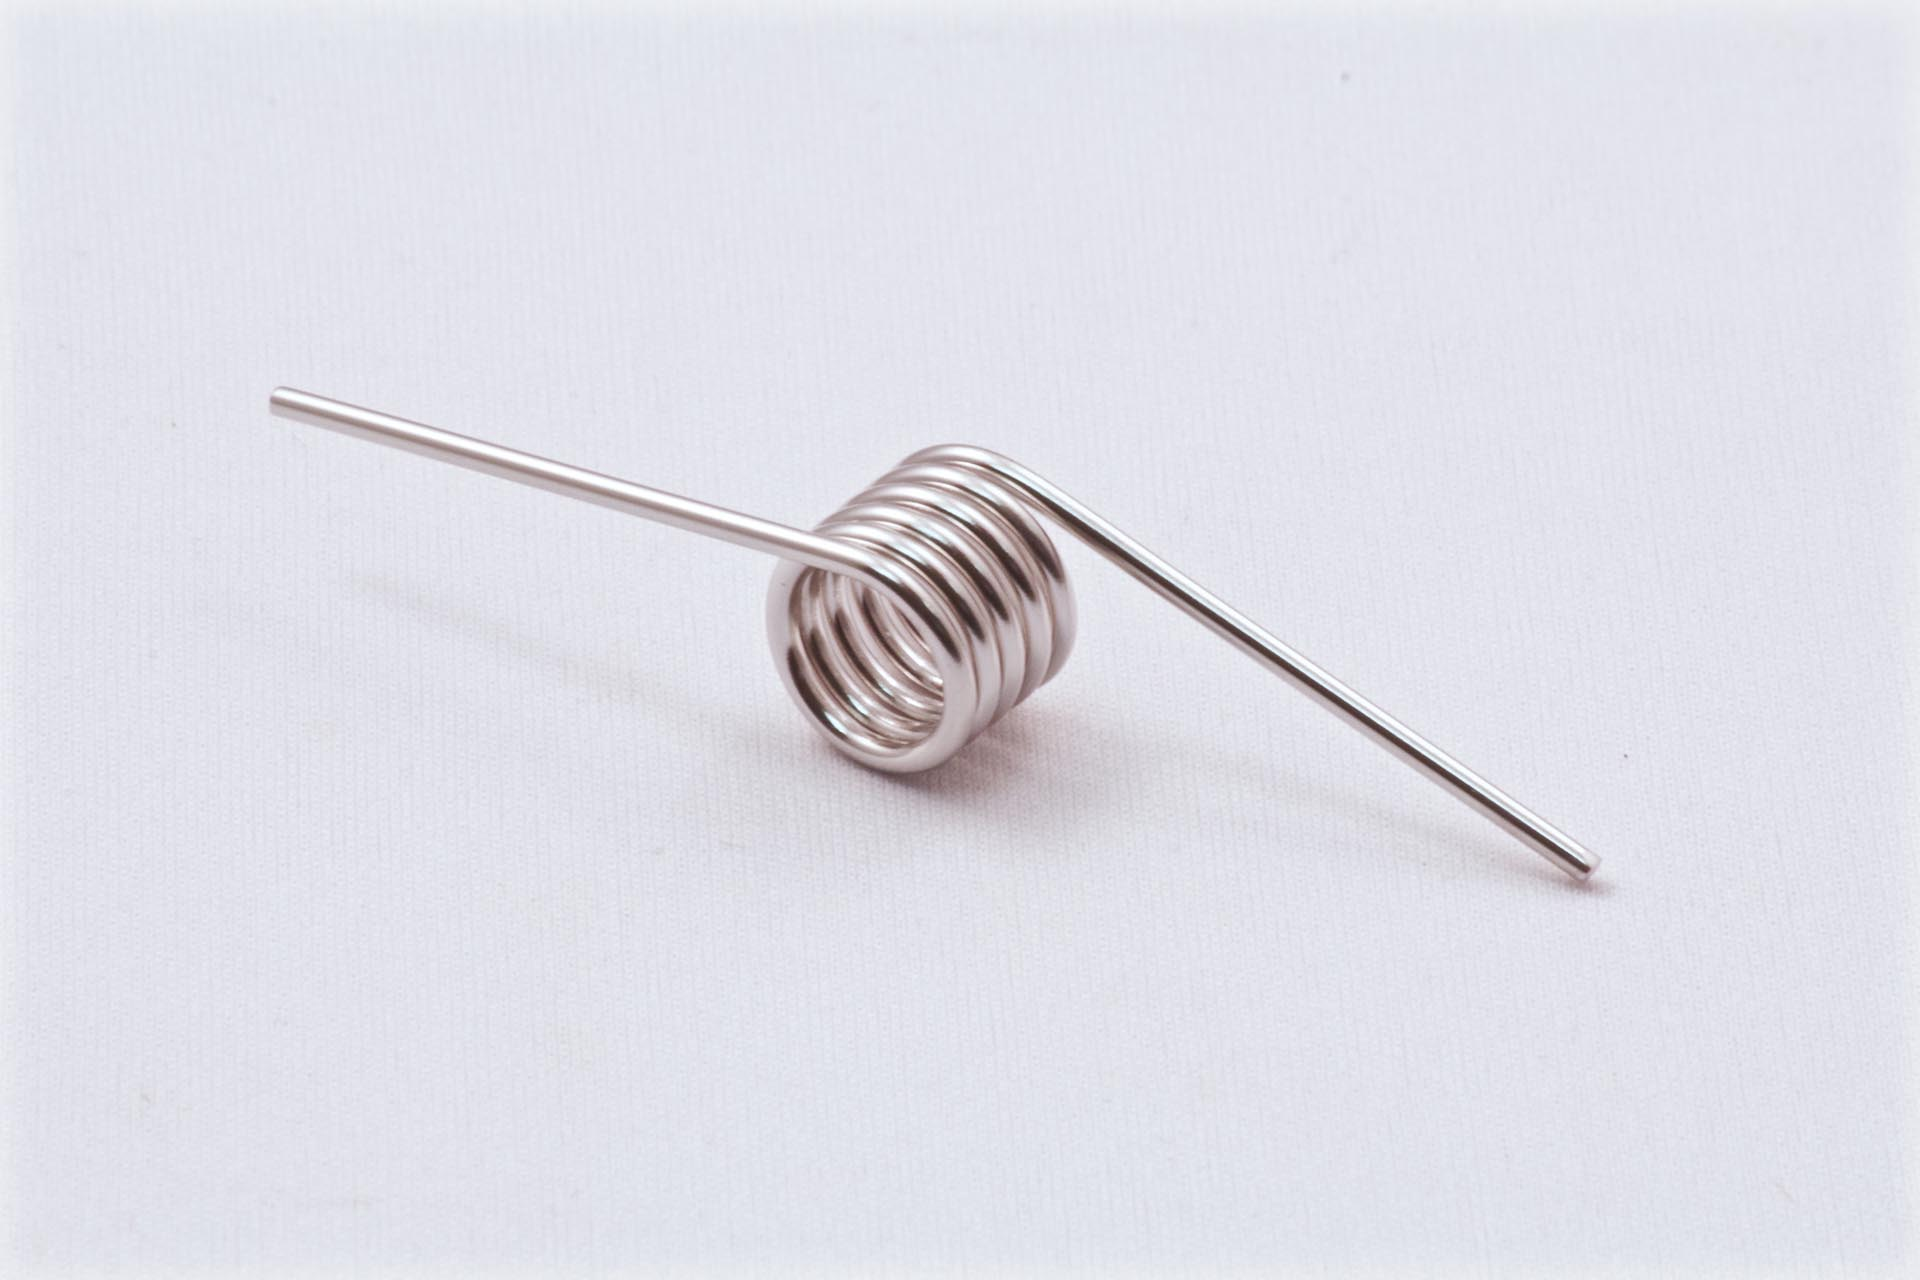
\includegraphics[width=0.45\textwidth]{torsion_spring.jpg}
        \caption{Torsieveer}
        \label{fig:torsieveer}
    \end{subfigure}
    \caption{Vraag over veren \& oscillatie}
\end{figure}

\subsection*{Oplossing}
\begin{figure}[H] 
    \centering
        \includegraphics[width=0.75\textwidth]{opl_torsieveer.pdf}

\end{figure}

\newpage 
\section*{Optie 3: James Bond in de achtervolging}
\subsection*{Opgave}
James Bond is in een achtervolging met een schurk. Beide rijden aan een constante snelheid $v$ over een vlak wegdek. Op een gegeven moment staat er een helling met hoek $\theta$ op hun pad (zie figuur \ref{fig:Bond},1). De helling heeft een hoogte $h_0$. De massa van James Bond en zijn Astin Martin is $M$ en die van de schurk en zijn vluchtwagen is $2M$. Beschouw beide auto's als puntmassa's. Gedurende de hele oefening mag wrijving verwaarloosd worden.
\begin{enumerate}[label=(\alph*)]
    \item De schurk rijdt over de helling en maakt een parabolische beweging (zie figuur \ref{fig:Bond}.2). Wat is het hoogste punt dat de schurk bereikt? Geef $x$- en $y$-coördinaten van dit punt op zijn traject. Veronderstel dat de snelheid van de schurk constant blijft terwijl hij de helling op rijdt.
    \item Op zijn hoogste punt vuurt de schurk een kogel af met massa $m$ onder een hoek $\theta$, zoals getekend in figuur \ref{fig:Bond}.3. Op dat moment rijdt ook James Bond op de helling. Met welke snelheid moet de kogel afgevuurd worden zodat James Bond geraakt wordt? Veronderstel dat de snelheid van James Bond constant blijft terwijl hij de helling op rijdt.
    \item Stel nu dat de schurk nog kon stoppen voor hij de helling op rijdt. James Bond kon echter niet op tijd stoppen en botst met een snelheid $v$ tegen de auto van de schurk. De botsing verloopt volledig elastisch. Bereken de snelheden van James Bond en de schurk net na de botsing. 
\end{enumerate}

\begin{figure}[H]
    \centering
    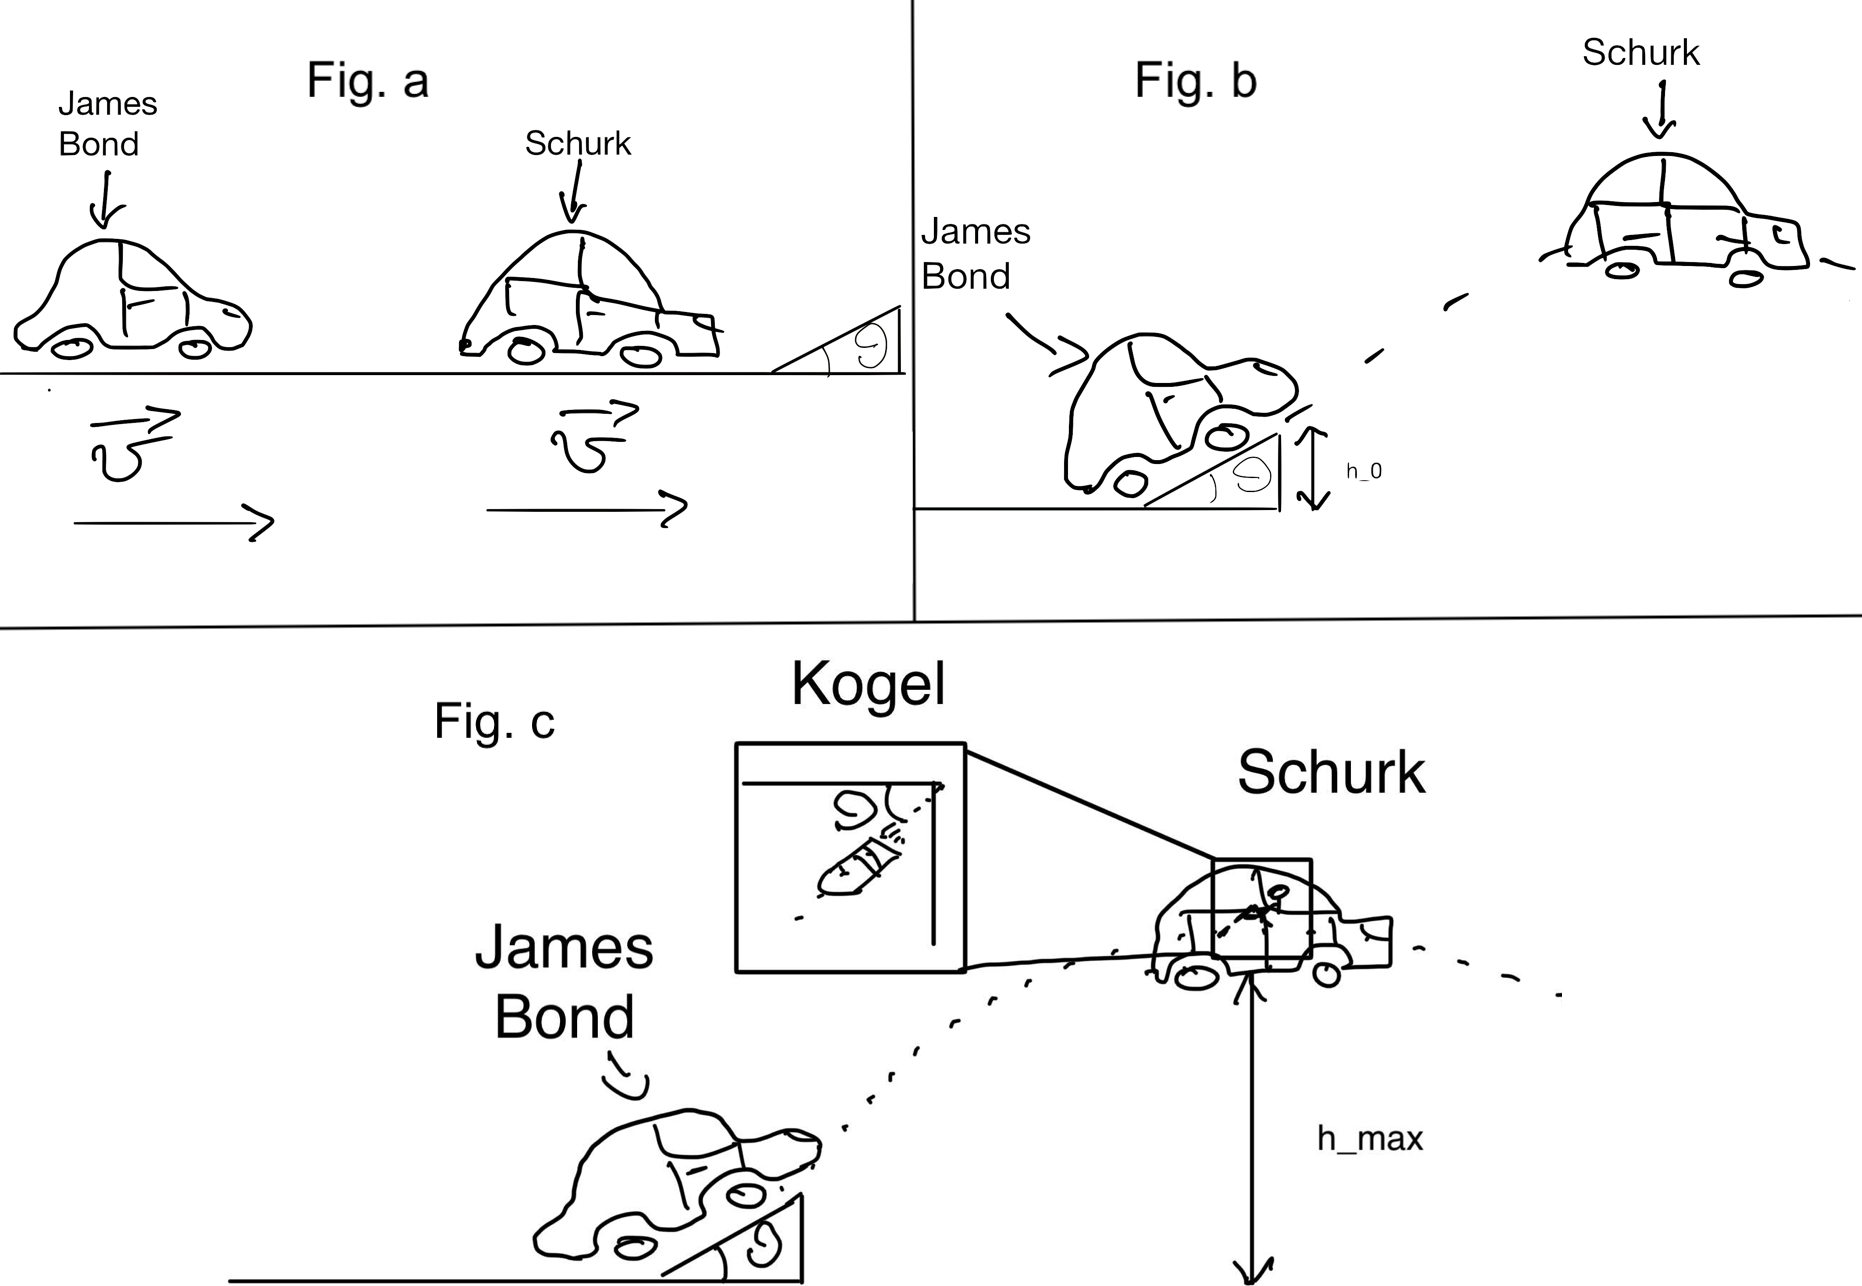
\includegraphics[width = \textwidth]{James_Bond.png} 
    \caption{}
    \label{fig:Bond}
\end{figure}

\subsection*{Oplossing}

\begin{enumerate}[label=(\alph*)]

    \item We beginnen met de bewegingsvergelijkingen op te stellen voor de vluchtwagen
    \begin{equation}
        x = x_0 + v_x t + a t^2 /2 = v_{x0} t,
    \end{equation}
    \begin{equation}
        y = y_0 + v_y t + a t^2 /2 = h_0 + v_{y0} t - gt^2/2.
    \end{equation}
    De componenten van de snelheid zijn
    \begin{equation}
        v_{x0} = \cos(\theta) v \text{ en } v_{y0} = \sin(\theta) v.
    \end{equation}
    Op het hoogste punt is de snelheid in de y-richting gelijk aan nul. Dus afleiden van vgl. (2) geeft
    \begin{equation}
        \begin{split}
            \frac{dy}{dt} &= 0 = v_{y0} - gt,\\
            &\Rightarrow t = v_{y0} / g,
        \end{split}
    \end{equation}
    het tijdstip waarop de schurk zijn hoogste punt bereikt. Dus het hoogste punt heeft een hoogte van 
    \begin{equation}
        \begin{split}
            y_{\text{max}} &= h_0 + v_{y0} t - gt^2/2 = h_0 + v_{y0}^2 / g - g/2 (v_{y0}^2 / g^2),\\
            & = h_0 + v_{y0}^2 / (2g).
        \end{split}
    \end{equation}
    op een afstand van 
    \begin{equation}
        x_{\text{max}} = v_{x0} t = v_{x0} v_{y0}/g = 2 \sin(2\theta)v^2/g,
    \end{equation}
    waar we voor de laatste gelijkheid gebruik hebben gemaakt van vgl. (3).

    \item Als de kogel James Bond raakt, moeten de x- en y-componenten van de beweginsvergelijkingen van James Bond en de kogel op een bepaald moment gelijk zijn aan elkaar. De bewegingsvergelijkingen voor James Bond zijn gelijk aan deze van de schurk en gegeven in vgl. (1) en (2).\\
    De vergelijkingen voor de kogel zijn de volgende
    \begin{equation}
        x_k = x_{\text{max}} - (u_{x0}-v_{x,\text{max}})t,
    \end{equation}
    \begin{equation}
        y_k = y_{\text{max}} - (u_{y0}-v_{y,\text{max}})t - gt^2/2,
    \end{equation}
    waarbij het minteken bij de snelheid aangeeft dat de kogel in tegengestelde richting is afgevuurd dan de auto rijdt.\\
    Hierbij weten we ook dat 
    \begin{equation}
        \begin{split}
           v_{x,\text{max}} &= v_{x0},\\
           v_{y,\text{max}} &= 0,
        \end{split}
    \end{equation}
    en voor de snelheid $u$ geldt ook
    \begin{equation}
        u_{x0} = \cos(\theta) u \text{ en } u_{y0} = \sin(\theta) u.
    \end{equation}
    We zoeken eerst het tijdstip van botsing via de x-richting
    \begin{align}
    	&&x_{\text{JB}} =& x_{\text{k}},\\
        \Rightarrow&& v_{x0} t =& v_{x0} v_{y0}/g - (u_{x0}-v_{x,\text{max}})t,\\
        \Rightarrow&&t =& v_{x0} v_{y0}/(gu_{x0}).
    \end{align}
    Dit invullen in de gelijkheid voor de y-richting geeft dan
    \begin{align}
            &&y_{\text{JB}} =& y_{\text{k}},\\
            \Rightarrow&& h_0 + v_{y0} t - gt^2/2 =& h_0 + v_{y0}^2 / (2g) - u_{y0}t- gt^2/2,\\
            \Rightarrow&&v_{y0} v_{x0} v_{y0}/(gu_{x0}) =& v_{y0}^2 / (2g) - u_{y0} v_{x0} v_{y0}/(gu_{x0}),\\
            \Rightarrow&&2v_{y0} v_{x0} =& v_{y0} u_{x0} - 2u_{y0} v_{x0} ,\\
            \Rightarrow&&2\sin(\theta) v \cos(\theta) v =& \sin(\theta) v \cos(\theta) u - 2 \sin(\theta) u \cos(\theta) v,\\
            \Rightarrow&&2v^2 =& vu - 2 uv,\\
            \Rightarrow&&2v^2 =& - uv,\\
             \Rightarrow&&u =& - 2v.\\
    \end{align}
    \item 
        Behoud van impuls geeft
        \begin{equation}
            M\boldsymbol{v} = M\boldsymbol{u_{\mathrm{JB}}} + 2M\boldsymbol{u_{\mathrm{s}}} \Rightarrow \boldsymbol{u_{\mathrm{JB}}} = \boldsymbol{v} - 2\boldsymbol{u_{\mathrm{s}}}.
        \end{equation}
        Behoud van energie geeft
        \begin{equation}
            Mv^2/2 = Mu_{\mathrm{JB}}^2/2 + 2Mu_{\mathrm{s}}^2/2 \Rightarrow v^2 = u_{\mathrm{JB}}^2 + 2u_{\mathrm{s}}^2.
        \end{equation}
        Invullen van vgl. (14) geeft dan
        \begin{align}
            &&v^2 &= (v^2 - 4\boldsymbol{u_{\mathrm{s}}} \boldsymbol{v} + 4u_{\mathrm{s}}^2) + 2u_{\mathrm{s}}^2,\\
            \Rightarrow&&4\boldsymbol{u_{\mathrm{s}}} \boldsymbol{v} & = 6u_{\mathrm{s}}^2.\\
            \Rightarrow&&u_{\mathrm{s}}v \cos(\phi) &= 3u_{\mathrm{s}}^2/2,\\
            \Rightarrow&&u_{\mathrm{s}} &= 2v/3.
        \end{align}
        En dus $u_{\mathrm{JB}} = -1v/3$.
\end{enumerate}



\newpage
\section*{Optie 4: Traagheidsmomenten \& energie}
\subsection*{Opgave}
Er worden drie objecten met constante massadichtheid $\sigma$ geroteerd met hoeksnelheid $\omega$ rondom een punt $P$. De eerste is een massieve schijf met als middelpunt $P$ en als straal $R$ (zie figuur \ref{fig:Schijf1}). De tweede is een massieve schijf met straal $R/2$ die rechts van het punt $P$ ligt (zie figuur \ref{fig:Schijf2}). De derde schijf is schijf 1, waar schijf 2 uit weggehaald werd (zie figuur \ref{fig:Schijf3}).
\begin{enumerate}[label=(\alph*)]
	\item Toon aan wat de traagheidsmomenten $I_1,I_2$ en $I_3$ zijn van de eerste, tweede en derde schijf respectievelijk.
	\item Toon aan dat de kinetische energie van de rotatie van schijf 1 gelijk is aan de som van kinetische energie\"en van de andere twee schijven.
\end{enumerate}
\begin{figure}[H]
	\centering
	\begin{subfigure}[b]{0.25\textwidth}
		\centering
		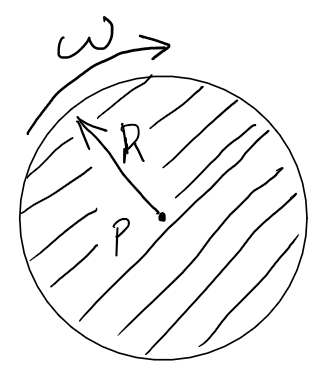
\includegraphics[width=\textwidth]{Schijf1}
		\caption{}
		\label{fig:Schijf1}
	\end{subfigure}
	\hfill
	\begin{subfigure}[b]{0.25\textwidth}
		\centering
		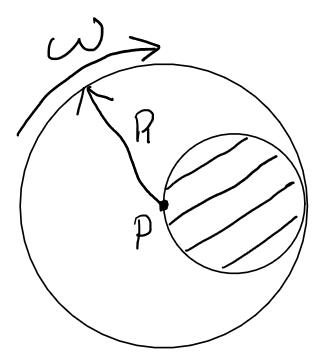
\includegraphics[width=\textwidth]{Schijf2}
		\caption{}
		\label{fig:Schijf2}
	\end{subfigure}
	\hfill
	\begin{subfigure}[b]{0.25\textwidth}
		\centering
		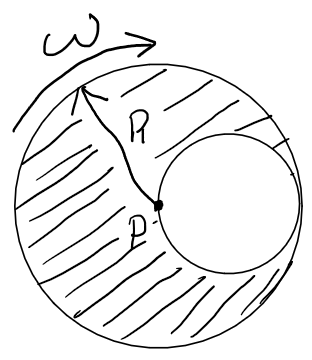
\includegraphics[width=\textwidth]{Schijf3}
		\caption{}
		\label{fig:Schijf3}
	\end{subfigure}
	\caption{Dit zijn drie verschillende objecten (gearceerde delen) die met hoeksnelheid $\omega$ geroteerd worden rondom punt $P$.}
	\label{fig:Schijven}
\end{figure}

\subsection*{Oplossing}
Schijf 1 draait gewoon rondom zijn COM dus we krijgen dat
\begin{equation}
	I_1=m_1R^2=2\pi \sigma R^4
\end{equation}
Voor schijf 2 krijgen we dat als die rondom zijn COM zou draaien dat dan
\begin{equation}
	\tilde I_2=m_2\left(\frac{R}{2}\right)^2=2\pi \sigma \left(\frac{R}{2}\right)^4=\frac{\pi}{8}\sigma R^4.
\end{equation}
Als we nu de parallele axis theorem (of Huygens–Steiner theorem) gebruiken krijgen we
\begin{equation}
	I_2=\frac{\pi}{8}\sigma R^4+m_2 \left(\frac{R}{2}\right)^2=\frac{\pi}{4}\sigma R^4.
\end{equation}
Het traagheidsmoment van van de laatste figuur is simpelweg het verschil tussen de andere twee
\begin{equation}\label{eq:I3IsI1MinI2}
	I_3=I_1-I_2=\frac{7\pi}{4}\sigma R^4.
\end{equation}
De laatste vraag is triviaal. Dit is omdat als we vergelijking \eqref{eq:I3IsI1MinI2} gebruiken, we krijgen dat:
\begin{align}
	E_2+E_3&=\frac{I_2\omega^2}{2}+\frac{I_3\omega^2}{2}\\
	&=\frac{(I_2+I_3)\omega^2}{2}\\
	&=\frac{I_1\omega^2}{2}=E_1.
\end{align}

\newpage

\end{document}